\documentclass{zkdl-presentation-template}

% Bibliography
\usepackage[
  backend=biber,
  style=alphabetic
]{biblatex} % Or your existing biblatex setup
\bibliography{bibliography.bib}

\usepackage{tabularx}

% Include subfigure package
\usepackage{subfigure}
\usepackage{subcaption}

% --- Some tikz functions ---
\newbox\dumbox
\newcommand{\mymark}[2]{%
  \setbox\dumbox=\hbox{#2}%
  \hbox to \wd\dumbox{\hss%
    \tikz[overlay,remember picture,baseline=(#1.base)]{ \node (#1) {\box\dumbox}; }%
    \hss}%
}

%% -- Draw small coefficient
\newcommand{\mysmall}[1]{%
  \tikz[overlay,remember picture]{%
    \node[blue,scale=.5, shift={(0,-.1)}] {$\times$#1};%
  }%
}

% Numeration
\addtobeamertemplate{navigation symbols}{}{%
    \usebeamerfont{footline}%
    \usebeamercolor[fg]{footline}%
    \hspace{1em}%
    \textbf{\insertframenumber/\inserttotalframenumber}
    \vspace{3.5px}
}

\title[Мережі Колмогорова-Арнольда]{\textbf{Застосування мереж
Колмогорова-Арнольда до задач комп'ютерного зору}} 

\author{Виконав: Захаров Д.О.\inst{1} \\ 
Науковий керівник: Ігнатович С.Ю.\inst{2}\\
Рецензент: Волощук О.Б.\inst{3}} 

\institute[shortinst]{
    \inst{1} Студент групи МП41 IV курсу (перший бакалаврський рiвень), спецiальностi 113
``Прикладна математика'' освiтньої програми ``Прикладна математика''.\\
    \inst{2} Доктор фiз.-мат. наук, професор кафедри прикладної математики. \\
    \inst{3} Доцент кафедри штучного інтелекту Харківського національного університету радіоелектроніки.\\
}

\date{12 червня, 2025}

\begin{document}
    \frame {
      \titlepage 
      %\hfill\includegraphics[trim={1.75cm 2.0cm 3.75cm 1cm},clip,width=0.4\textwidth]{../code/classification-cont-prediction.pdf}
    }
  
    % \begin{frame}{План}
    %   \tableofcontents
    % \end{frame}

    \section[Вступ]{Вступ: навіщо нам KAN?}

    \subsection{Актуальність задачі}
    \begin{frame}{Опис типової задачі}
        \begin{itemize}
            \item На вхід подається певний набір даних $\mathcal{D}$.
            Найчастіше, це набір пар $\{(\boldsymbol{x}_n,\boldsymbol{y}_n)\}_{1
            \leq n \leq N} \subseteq \mathcal{X} \times \mathcal{Y}$ (\textit{supervised learning}).
            \item Часто ми хочемо знайти так звану \textit{модель} $f:
            \mathcal{X} \to \mathcal{Y}$, для якої $f(\boldsymbol{x}_n) \approx
            \boldsymbol{y}_n$: ми передбачаємо значення $\boldsymbol{y}_n$ на
            основі $\boldsymbol{x}_n$.
            \item Функцію $f$ ми маємо підібрати з певного класу $\mathcal{F}$
            так, щоб за неї досягався певний мінімум ($\widehat{f} := \argmin_{f
            \in \mathcal{F}}\mathcal{L}(\mathcal{D}|f)$).
        \end{itemize}

        \begin{block}{Ціль дипломної роботи}
            \begin{itemize}[label={$\checkmark$}]
                \item Зараз $\mathcal{F}$ --- це параметризоване сімейство MLP
                архітектур нейронних мереж. В роботі, ми дослідили, чому такий
                вибір взагалі працює на практиці.
                \item Ми дослідили альтернативну парадигму вибору $\mathcal{F}$
                --- мережі Колмогорова-Арнольда (KAN), а також розширили
                конструкцію KAN на конволюційні нейронні мережі.
            \end{itemize}
        \end{block}
    \end{frame}

    \begin{frame}{Задача машинного навчання: приклад}
    \vspace{-17.5px}
    \begin{equation*}
        \textbf{Задача}: \textcolor{blue!90!black}{\hat{\boldsymbol{\theta}} := \argmin_{\boldsymbol{\theta} \in \Theta} \mathcal{L}(\mathcal{D}|f_{\boldsymbol{\theta}})} \; \text{де} \;
        \textcolor{green!50!black}{f_{\theta}(\boldsymbol{x}) = \theta_0+\sum_{i=1}^n \theta_ix_i}
    \end{equation*}
    \vspace{-10px}
    \begin{figure}
        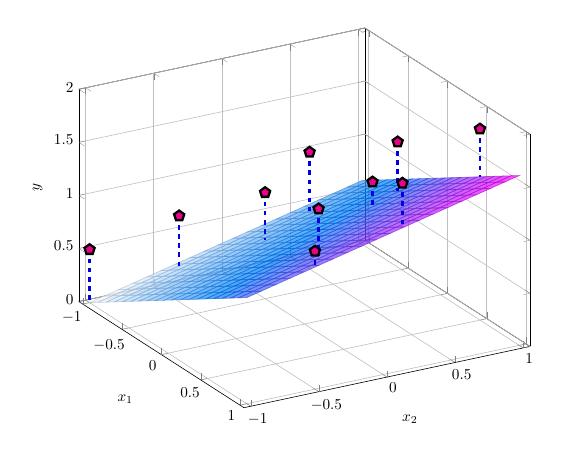
\begin{tikzpicture}[scale=0.55]
            % Define the 3D plot
            \begin{axis}[
                view={60}{30}, % Angle for 3D view
                xlabel={$x_1$},
                ylabel={$x_2$},
                zlabel={$y$},
                domain=-1:1,
                samples=20,
                width=12cm,
                grid=both,
                zmin=0, zmax=2,
                xmin=-1.05, xmax=1.05,
                ymin=-1.05, ymax=1.05,
                colormap/cool
            ]
        
            % Plot the regression plane
            \addplot3[surf, opacity=0.7] {0.5*x + 0.3*y + 0.8};
        
            % Add sample data points
            \addplot3[only marks, mark=pentagon*, fill=magenta, mark size=3.5pt, line width=1.5pt] coordinates {
                (-1, -1, 0.5)
                (-0.8, 0.5, 1.1)
                (-0.5, 0, 1)
                (-0.2, 0.8, 1.4)
                (0, 0.5, 1.2)
                (0.5, 1, 1.8)
                (0.7, -0.3, 1.5)
                (0.9, 0.2, 1.7)
                (1, -0.5, 1.3)
                (-0.9, -0.4, 0.7)
            };
        
            % Add red dashed projection lines without labels
            \addplot3[blue!90!black, ultra thick, dashed] coordinates {(-1, -1, 0.5) (-1, -1, {0.5*-1 + 0.3*-1 + 0.8})};
            \addplot3[blue!90!black, ultra thick, dashed] coordinates {(-0.8, 0.5, 1.1) (-0.8, 0.5, {0.5*-0.8 + 0.3*0.5 + 0.8})};
            \addplot3[blue!90!black, ultra thick, dashed] coordinates {(-0.5, 0, 1) (-0.5, 0, {0.5*-0.5 + 0.3*0 + 0.8})};
            \addplot3[blue!90!black, ultra thick, dashed] coordinates {(-0.2, 0.8, 1.4) (-0.2, 0.8, {0.5*-0.2 + 0.3*0.8 + 0.8})};
            \addplot3[blue!90!black, ultra thick, dashed] coordinates {(0, 0.5, 1.2) (0, 0.5, {0.5*0 + 0.3*0.5 + 0.8})};
            \addplot3[blue!90!black, ultra thick, dashed] coordinates {(0.5, 1, 1.8) (0.5, 1, {0.5*0.5 + 0.3*1 + 0.8})};
            \addplot3[blue!90!black, ultra thick, dashed] coordinates {(0.7, -0.3, 1.5) (0.7, -0.3, {0.5*0.7 + 0.3*-0.3 + 0.8})};
            \addplot3[blue!90!black, ultra thick, dashed] coordinates {(0.9, 0.2, 1.7) (0.9, 0.2, {0.5*0.9 + 0.3*0.2 + 0.8})};
            \addplot3[blue!90!black, ultra thick, dashed] coordinates {(1, -0.5, 1.3) (1, -0.5, {0.5*1 + 0.3*-0.5 + 0.8})};
            \addplot3[blue!90!black, ultra thick, dashed] coordinates {(-0.9, -0.4, 0.7) (-0.9, -0.4, {0.5*-0.9 + 0.3*-0.4 + 0.8})};

            % Label axes
            %\node at (axis cs: 1, 0, 2) [anchor=north west] {Regression Plane};
            %\node at (axis cs: -1, -1, 0) [anchor=north] {Data Points};
            %\node at (axis cs: -1, 1, 1.5) [anchor=west, rotate=15] {Error Lines (Loss)};
            
            \end{axis}
        \end{tikzpicture}
        \caption{Приклад багатовимірної лінійної регресії для $\boldsymbol{x}_n
        \in \mathbb{R}^2$, $y_n \in \mathbb{R}$. Ціль підібрати площину
        $f(\boldsymbol{x}|\beta,w_1,w_2) := \beta+w_1x_1+w_2x_2$ так, щоб
        втрата $\mathcal{L}(\mathcal{D}|\beta,w_1,w_2)=\frac{1}{N}\sum_{n=1}^N\textcolor{blue!90!black}{\|f(\boldsymbol{x}_n) -
        y_n\|^2}$ була мінімальною.}
    \end{figure}
    \end{frame}

    \begin{frame}{Актуальність нейронних мереж}
        У попередніх наших роботах
        \cite{our-biometrics-1,our-biometrics-2,our-biometrics-3} ми, зокрема,
        досліджували задачу кібербезпеки біометричних даних:

        \begin{table}
            \scriptsize
            \centering
            \begin{tabularx}{\textwidth}{|c|X|X|X|}
                \hline
                \cellcolor{gray!20}\textbf{Робота} & \cellcolor{gray!20}\textbf{Рік, Журнал} & \cellcolor{gray!20}\textbf{Модель} & \cellcolor{gray!20}\textbf{Набір даних} \\
                \cite{our-biometrics-1} & 2023, Multimedia Tools and Applications (Springer) & $f: \mathcal{I} \to \{0,1\}^{128}$: Бінарний вектор характеристик & Зображення та ідентифікатори людей \\
                \cite{our-biometrics-2} & 2024, Computers \& Security (Elsevier) & $f: \mathcal{I} \to \{0,1\}$: Класифікатор живності & Зображення та біти ``фейк/не фейк'' \\
                \cite{our-biometrics-3} & 2024, Engineering Applications of AI (Elsevier) & $f: \mathcal{I} \to \mathcal{I}$: ``Геш'' значення фотографії людини & Зображення та ідентифікатори людей \\
                \hline
            \end{tabularx}
            \caption{Приклади наших робіт з біометрії. $\mathcal{I}$ --- множина зображень.}
        \end{table}

        \begin{alertblock}{Питання нашого дослідження}
            Зараз ці задачі розв'язуються за допомогою MLP парадигми. Чи є
            \textit{потенціал} у використанні KAN архітектур для розв'язання 
            подібних задач з комп'ютерного зору?
        \end{alertblock}
    \end{frame}

    \begin{frame}{Актуальність KAN архітектур}
        \begin{itemize}
            \item \textbf{``Плато'' LLM:} Згідно багатьом дослідженням (напр.
            ``On the Dangers of Stochastic Parrots: Can Language Models Be Too
            Big?''~\cite{dangers}), ми досягаємо деякого ``плато'' у розвитку
            нейронних мереж. Значить, нам потрібні нові підходи до побудови
            архітектур.
            \item \textbf{Кібербезпека та нейронні мережі:} У сфері
            кібербезпеки, актуальним питанням стає написання нейронних мереж у
            вигляді арифметичних ланцюгів (arithmetical circuits). Отже,
            потрібно досліджувати структури мереж, що можуть бути
            ``дружелюбними'' до таких арифметичних схем.
        \end{itemize}
        \begin{figure}
            \centering
            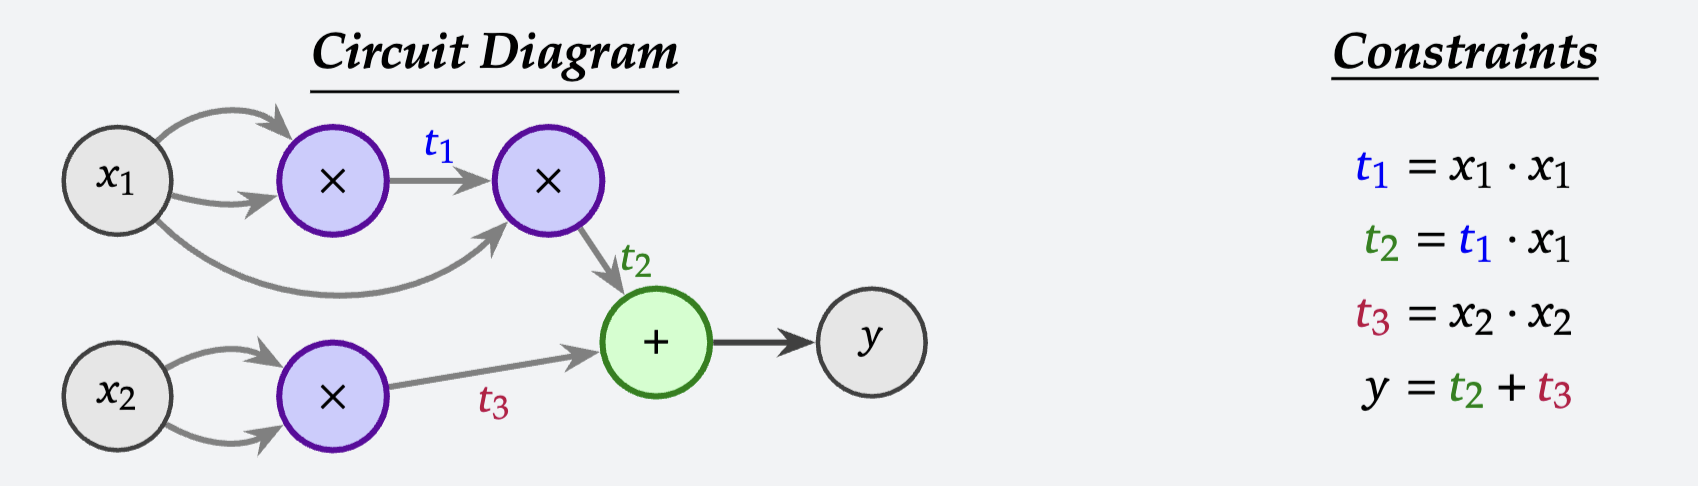
\includegraphics[width=0.8\textwidth]{images/circuits.png}
            \label{fig:kan-architecture}
        \end{figure}
    \end{frame}

    \section{MLP vs KAN}

    \subsection{Багатошарова Модель Персептронів (MLP)}

        \begin{frame}{MLP парадигма}
        Розглянемо сучасну парадигму побудов архітектур --- MLP.
        \begin{block}{Апроксимація функцій лінійною комбінацією сігмоїдів}
            Робота Цибенко \cite{cybenko} присвячена на той час відомій апроксимації функції $f:
            \mathbb{R}^m \to \mathbb{R}$ за допомогою наступної суми:
            \begin{equation*}\label{eq:cybenko-g}
                \hat{f}(\boldsymbol{x}) = \sum_{j=1}^n \alpha_j \sigma(\boldsymbol{w}_j^{\top}\boldsymbol{x} + \beta_j), \quad \sigma(-\infty) = 0,\; \sigma(+\infty) = 1,
            \end{equation*}
            \begin{itemize}
                \item По суті, лінійна комбінація виразів $\{\sigma(\boldsymbol{w}_j^{\top}\boldsymbol{x} + \beta_j)\}_{1 \leq j \leq n}$.
                \item $n$ --- кількість нейронів у прихованому шарі.
                \item Маємо $\mathcal{O}(mn)$ параметрів.
            \end{itemize}
            
        \end{block}

        \begin{alertblock}{Питання}
            Який клас функцій може апроксимувати така модель?
        \end{alertblock}
    \end{frame}

    \begin{frame}{Візуалізація Архітектури Цибенко}
        \begin{tikzpicture}[scale=0.8]
            % Define layers and node style
            \tikzset{input-neuron/.style={
                circle, 
                draw=green!80!black, 
                line width=0.5mm,
                fill=green!20!white,
                minimum size=0.5cm
            }}
            \tikzset{hidden-neuron/.style={
                circle, 
                draw=blue!80!black, 
                line width=0.5mm,
                fill=blue!20!white,
                minimum size=0.5cm
            }}
            \tikzset{output-neuron/.style={
                circle, 
                draw=orange!80!black, 
                line width=0.5mm,
                fill=orange!20!white,
                minimum size=0.5cm
            }}
            
            % Input layer
            \foreach \i in {1, 2, 3} {
                \node[input-neuron] (I\i) at (0, -1.25*\i) {$x_{\i}$};
            }
        
            % Hidden layer
            \foreach \j in {1, 2, 3, 4, 5} {
                \node[hidden-neuron] (h\j) at (4, -1.25*\j + 1.25) {$\Sigma$};
                \node[hidden-neuron] (H\j) at (6, -1.25*\j + 1.25) {$z_{\j}$};
                \draw[very thick,-{Stealth[length=3.5mm]}] (h\j) to [edge label=$\sigma$] (H\j);
            }
        
            % Output layer
            \node[output-neuron] (O) at (10, -2.5) {$\hat{f}(\boldsymbol{x})$};
        
            % Draw connections from input to hidden layer
            \foreach \i in {1, 2, 3} {
                \foreach \j in {1, 2, 3, 4, 5} {
                    \draw[very thick,-{Stealth[length=3.5mm]}] (I\i) -- (h\j);
                }
            }
        
            % Draw connections from hidden to output layer
            \foreach \j in {1, 2, 3, 4, 5} {
                \draw[very thick,-{Stealth[length=3.5mm]}] (H\j) -- (O);
            }
        
            % Labels
            \node[above, align=center] at (0, 0.5) {\textcolor{green!80!black}{\textbf{Вхідний шар}}\\$m$ нейронів};
            \node[above, align=center] at (5, 0.5) {\textcolor{blue!80!black}{\textbf{Прихований шар}}\\$n$ нейронів};
            \node[above, align=center] at (10, 0.5) {\textcolor{orange!80!black}{\textbf{Вихідний шар}}\\1 нейрон};
        
        \end{tikzpicture}
    \end{frame}

    \begin{frame}{Теорема Цибенко}
        \begin{itemize}
            \item $\mathcal{Q}_m = [0,1]^m$ є $m$-вимірним одиничним гіперкубом.
            \item $\mathcal{C}(\mathcal{Q}_m)$ --- простір неперервних функцій $f: \mathcal{Q}_m \to \mathbb{R}$.
            \item Норма функції $f$ на $\mathcal{C}(\mathcal{Q}_m)$: $\|f\|_{\mathcal{Q}_m} = \sup_{\boldsymbol{x} \in \mathcal{Q}_m} |f(\boldsymbol{x})|$.
        \end{itemize}

        \begin{theorem}[Цибенко]
            Нехай $\sigma$ будь-яка неперервна сігмоїдальна функція. Суми вигляду
            $\hat{f}(\boldsymbol{x}) = \sum_{j=1}^n
            \alpha_j\sigma(\boldsymbol{w}_j^{\top}\boldsymbol{x} + \beta_j)$ є щільними у
            $\mathcal{C}(\mathcal{Q}_m)$ та $L^1(\mathcal{Q}_m)$. Іншими словами, для
            будь-якої функції $f \in \mathcal{C}(\mathcal{Q}_m)$ та $\varepsilon > 0$,
            існує сума $\hat{f}(\boldsymbol{x})$ така, що:
            \begin{enumerate}
                \item $|\hat{f}(\boldsymbol{x})-f(\boldsymbol{x})|<\varepsilon$ для всіх $\boldsymbol{x} \in
                \mathcal{Q}_m$.
                \item $\int_{\mathcal{Q}_m}|\hat{f}(\boldsymbol{x})-f(\boldsymbol{x})|d\boldsymbol{x} <
                \varepsilon$.
            \end{enumerate}
        \end{theorem}

        \begin{alertblock}{Висновок}
            $\sum_{j=1}^n
            \alpha_j\sigma(\boldsymbol{w}_j^{\top}\boldsymbol{x} + \beta_j)$ апроксимує 
            довільну функцію на $\mathcal{C}(\mathcal{Q}_m)$.
        \end{alertblock}
    \end{frame}

    
    \begin{frame}{Практична реалізація}
        \begin{alertblock}{Додаток}
            У дипломній роботі ми написали програму, що для заданого бінарного
            розбиття $\mathcal{P}_0,\mathcal{P}_1$ квадрату $[0,1]^2$, будує
            оптимальний класифікатор $\hat{f}$.
        \end{alertblock}

        % Show two images side by side using minipage
        \begin{figure}
            \begin{minipage}{0.475\textwidth}
                \centering
                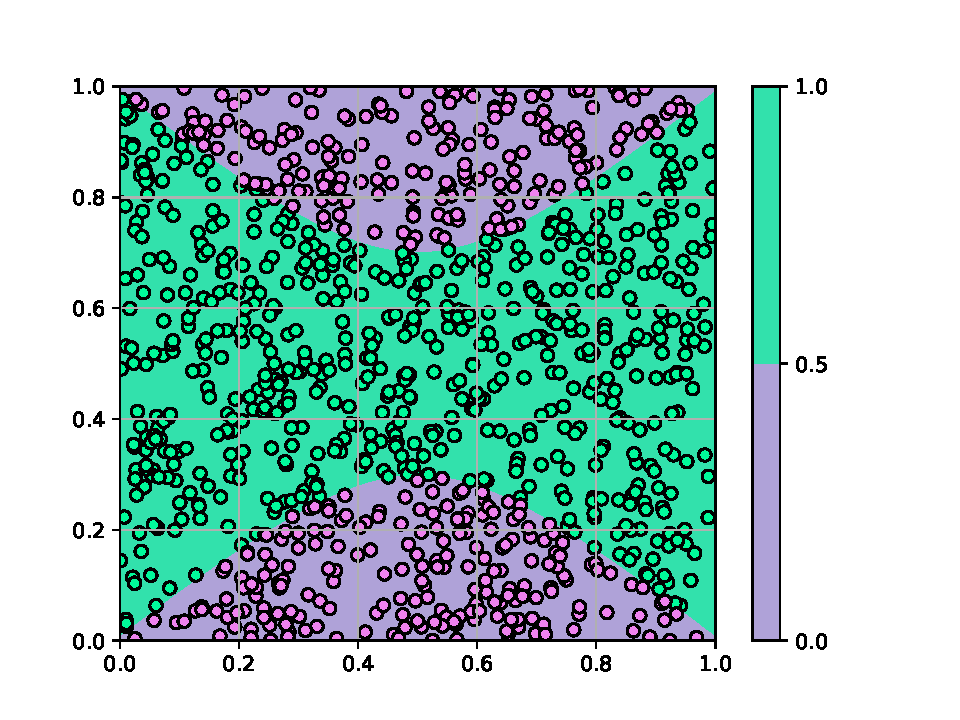
\includegraphics[width=\textwidth]{images/classification-example.pdf}
                \caption{Правильне розбиття квадрату $\mathcal{P}_0,\mathcal{P}_1$.}
            \end{minipage}\hfill
            \begin{minipage}{0.475\textwidth}
                \centering
                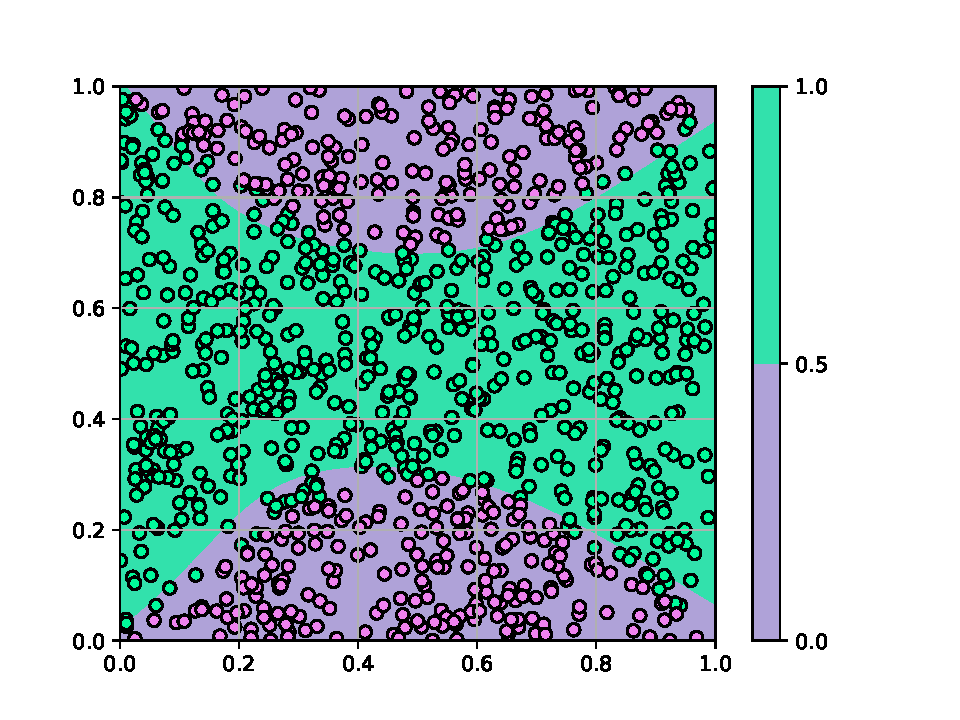
\includegraphics[width=\textwidth]{images/classification-discr-prediction.pdf}
                \caption{Розбиття, знайдене класифікатором $\hat{f}$.}
            \end{minipage}
        \end{figure}
    \end{frame}

    \begin{frame}{Узагальнення: MLP}
        \begin{enumerate}
            \item Замість сігмоїду $\sigma$, використовуються інші \textbf{нелінійні}
            активаційні функції $\phi: \mathbb{R} \to \mathbb{R}$ (напр., $\phi(x) = \max\{0,x\}$).
            \item Замість двох шарів, може бути довільна кількість шарів.
        \end{enumerate}

        \begin{definition}[Багатошарова модель персептронів (MLP)]\label{def:mlp}
            Таким чином, узагальнена архітектура:
            \begin{equation*}
                \boldsymbol{x}^{\langle j+1 \rangle} = \phi^{\langle j \rangle}(\boldsymbol{z}^{\langle j \rangle}), \quad \boldsymbol{z}^{\langle j \rangle} = \boldsymbol{W}^{\langle j \rangle}\boldsymbol{x}^{\langle j \rangle} + \boldsymbol{\beta}^{\langle j \rangle}, \quad j = 0,\dots,\ell-1,
            \end{equation*}
        \end{definition}

        \begin{alertblock}{Зауваження}
            У дипломній роботі, ми розглянули питання: (a) навіщо потрібно більше двох шарів, (b) які бувають узагальнення архітектури MLP та (c) навіщо інші активаційні функції.
        \end{alertblock}
    \end{frame}

    \subsection{Історична довідка: 13 проблема Гільберта}
    
    \begin{frame}{Теорема Колмогорова-Арнольда}
        \begin{block}{Основна гіпотеза 13 проблеми Гільберта}
            Існує неперервна функція $f: \mathcal{Q}_3 \to \mathbb{R}$, що не може бути
            виражена як композиція та сума неперервних функцій $\phi_1,\dots,\phi_N \in
            \mathcal{C}(\mathbb{R}^2)$.
        \end{block}

        Проте, у 1957 році Колмогоров показав обернене.

        \begin{definition}[Теорема Колмогорова (1957, \cite{kolmogorov-original})]
            Для будь-якого натурального $m \geq 2$, існують неперервні функції
            $\phi_{p,q} \in \mathcal{C}([0,1])$ такі, що для будь-якої функції $f \in
            \mathcal{C}(\mathcal{Q}_m)$ знайдуться неперервні функції
            $\Phi_1,\dots,\Phi_{2m+1} \in \mathcal{C}(\mathbb{R})$ такі, що
            \begin{equation*}
                f(x_1,\dots,x_m) = \sum_{q=1}^{2m+1}\Phi_q\left(\sum_{p=1}^m \phi_{p,q}(x_p)\right)
            \end{equation*}
        \end{definition}
    \end{frame}

    \subsection{Мережа Колмогорова-Арнольда}
    \begin{frame}{Мережа Колмогорова-Арнольда(KAN)}
        \begin{block}{Зауваження}
            До роботи 2024 року \cite{kan}, ідею такої репрезентації вважали недосяжною через
            ``поганість'' функцій $\phi_{p,q}$ та $\Phi_q$. 
        \end{block}

        \begin{definition}[З'єднання KAN Мережі \cite{kan}]
            \textbf{З'єднання KAN Мережі} між шарами розміру $n$ (вхід)
            та $m$ (вихід) --- це матриця $\boldsymbol{\Phi} = \{\phi_{q,p}\}_{1 \leq p \leq n, 1 \leq q \leq m}$, де 
            кожна функція параметризована, а наступне значення активації $\boldsymbol{y} = \boldsymbol{\Phi} \circ \boldsymbol{x}$.
        \end{definition}

        \begin{equation*}
            \begin{bmatrix}
                y_1 \\
                \vdots \\
                y_{m}
            \end{bmatrix} =
            \begin{bmatrix}
                \phi_{1,1} & \cdots & \phi_{1,n} \\
                \vdots & \ddots & \vdots \\
                \phi_{m,1} & \cdots & \phi_{m,n}
            \end{bmatrix}\circ \begin{bmatrix}
                x_1 \\
                \vdots \\
                x_n
            \end{bmatrix} \triangleq \begin{bmatrix}
                \sum_{p=1}^n \phi_{1,p}(x_p) \\
                \vdots \\
                \sum_{p=1}^n \phi_{m,p}(x_p)
            \end{bmatrix}
        \end{equation*}
    \end{frame}

    \begin{frame}{Мережа Колмогорова-Арнольда(KAN), cont.}
        \begin{definition}[Архітектура KAN \cite{kan}]
            \textbf{Мережа Колмогорова-Арнольда} --- це композиція $\ell$ з'єднань:
            \begin{equation*}
                \hat{f}_{\text{KAN}}(\boldsymbol{x}) = \boldsymbol{\Phi}^{\langle \ell-1 \rangle} \circ \cdots \circ \boldsymbol{\Phi}^{\langle 1 \rangle} \circ \boldsymbol{\Phi}^{\langle 0 \rangle} \circ \boldsymbol{x}.
            \end{equation*}
        \end{definition}

        \begin{figure}
            % Include figure
            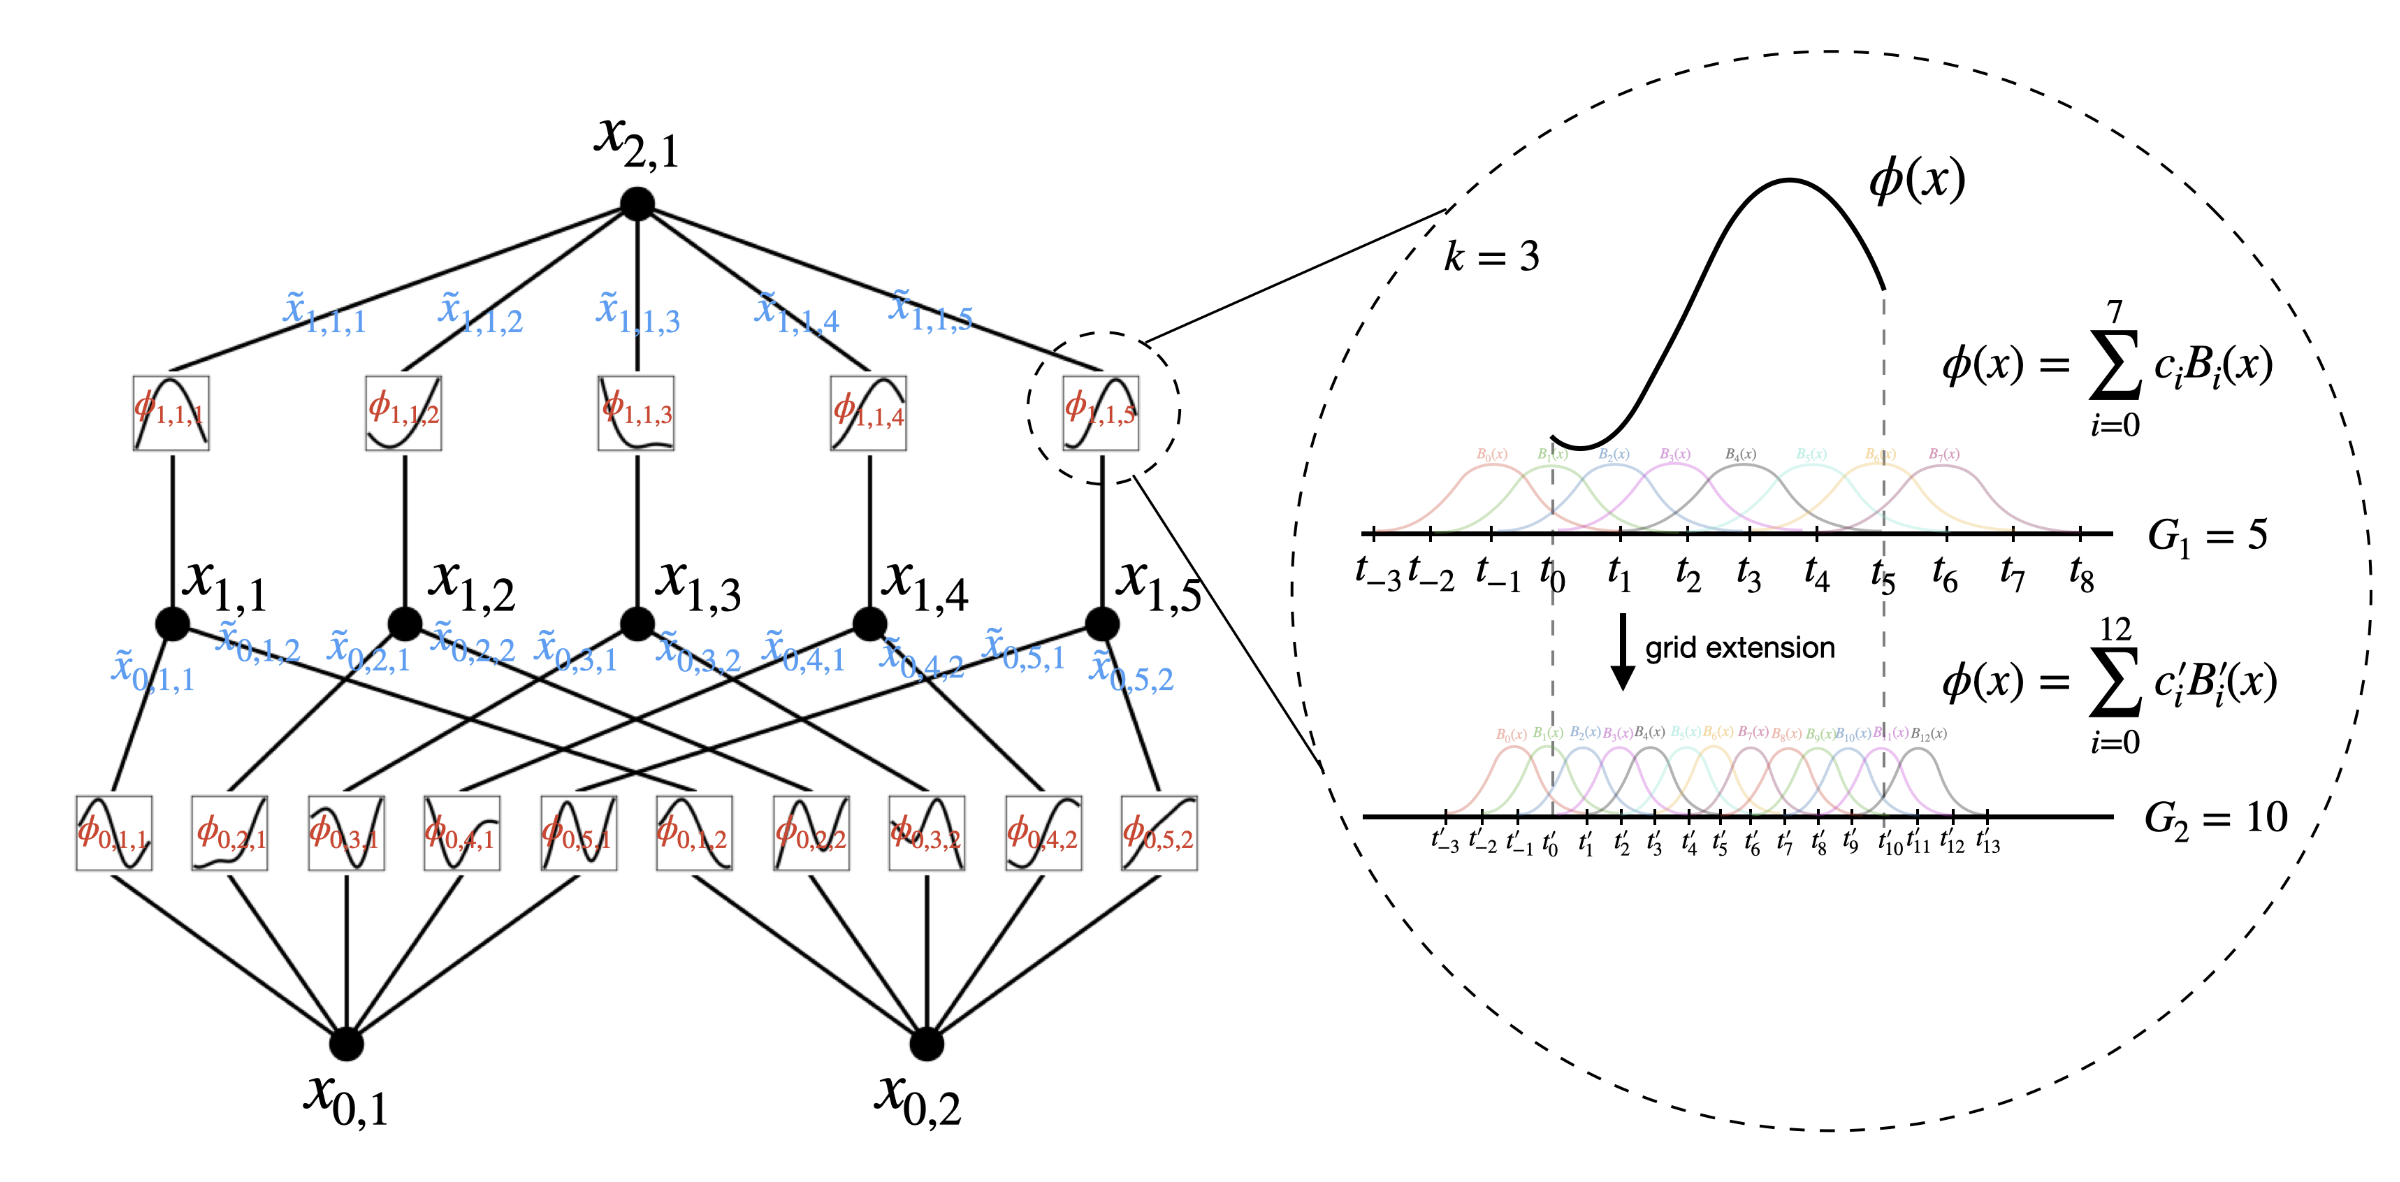
\includegraphics[width=0.8\textwidth]{images/kan.png}
            \caption{Архітектура мережі Колмогорова-Арнольда з оригінальної роботи \cite{kan}.}
        \end{figure}
    \end{frame}

    \begin{frame}{Інтерпретованість KAN}
        KAN мережі є дуже \textit{інтерпретованими} та \textit{застосовними в
        наукових задачах}: див. ретельне дослідження від авторів
        оригінальної роботи \cite{kan-2}.

        \begin{figure}
            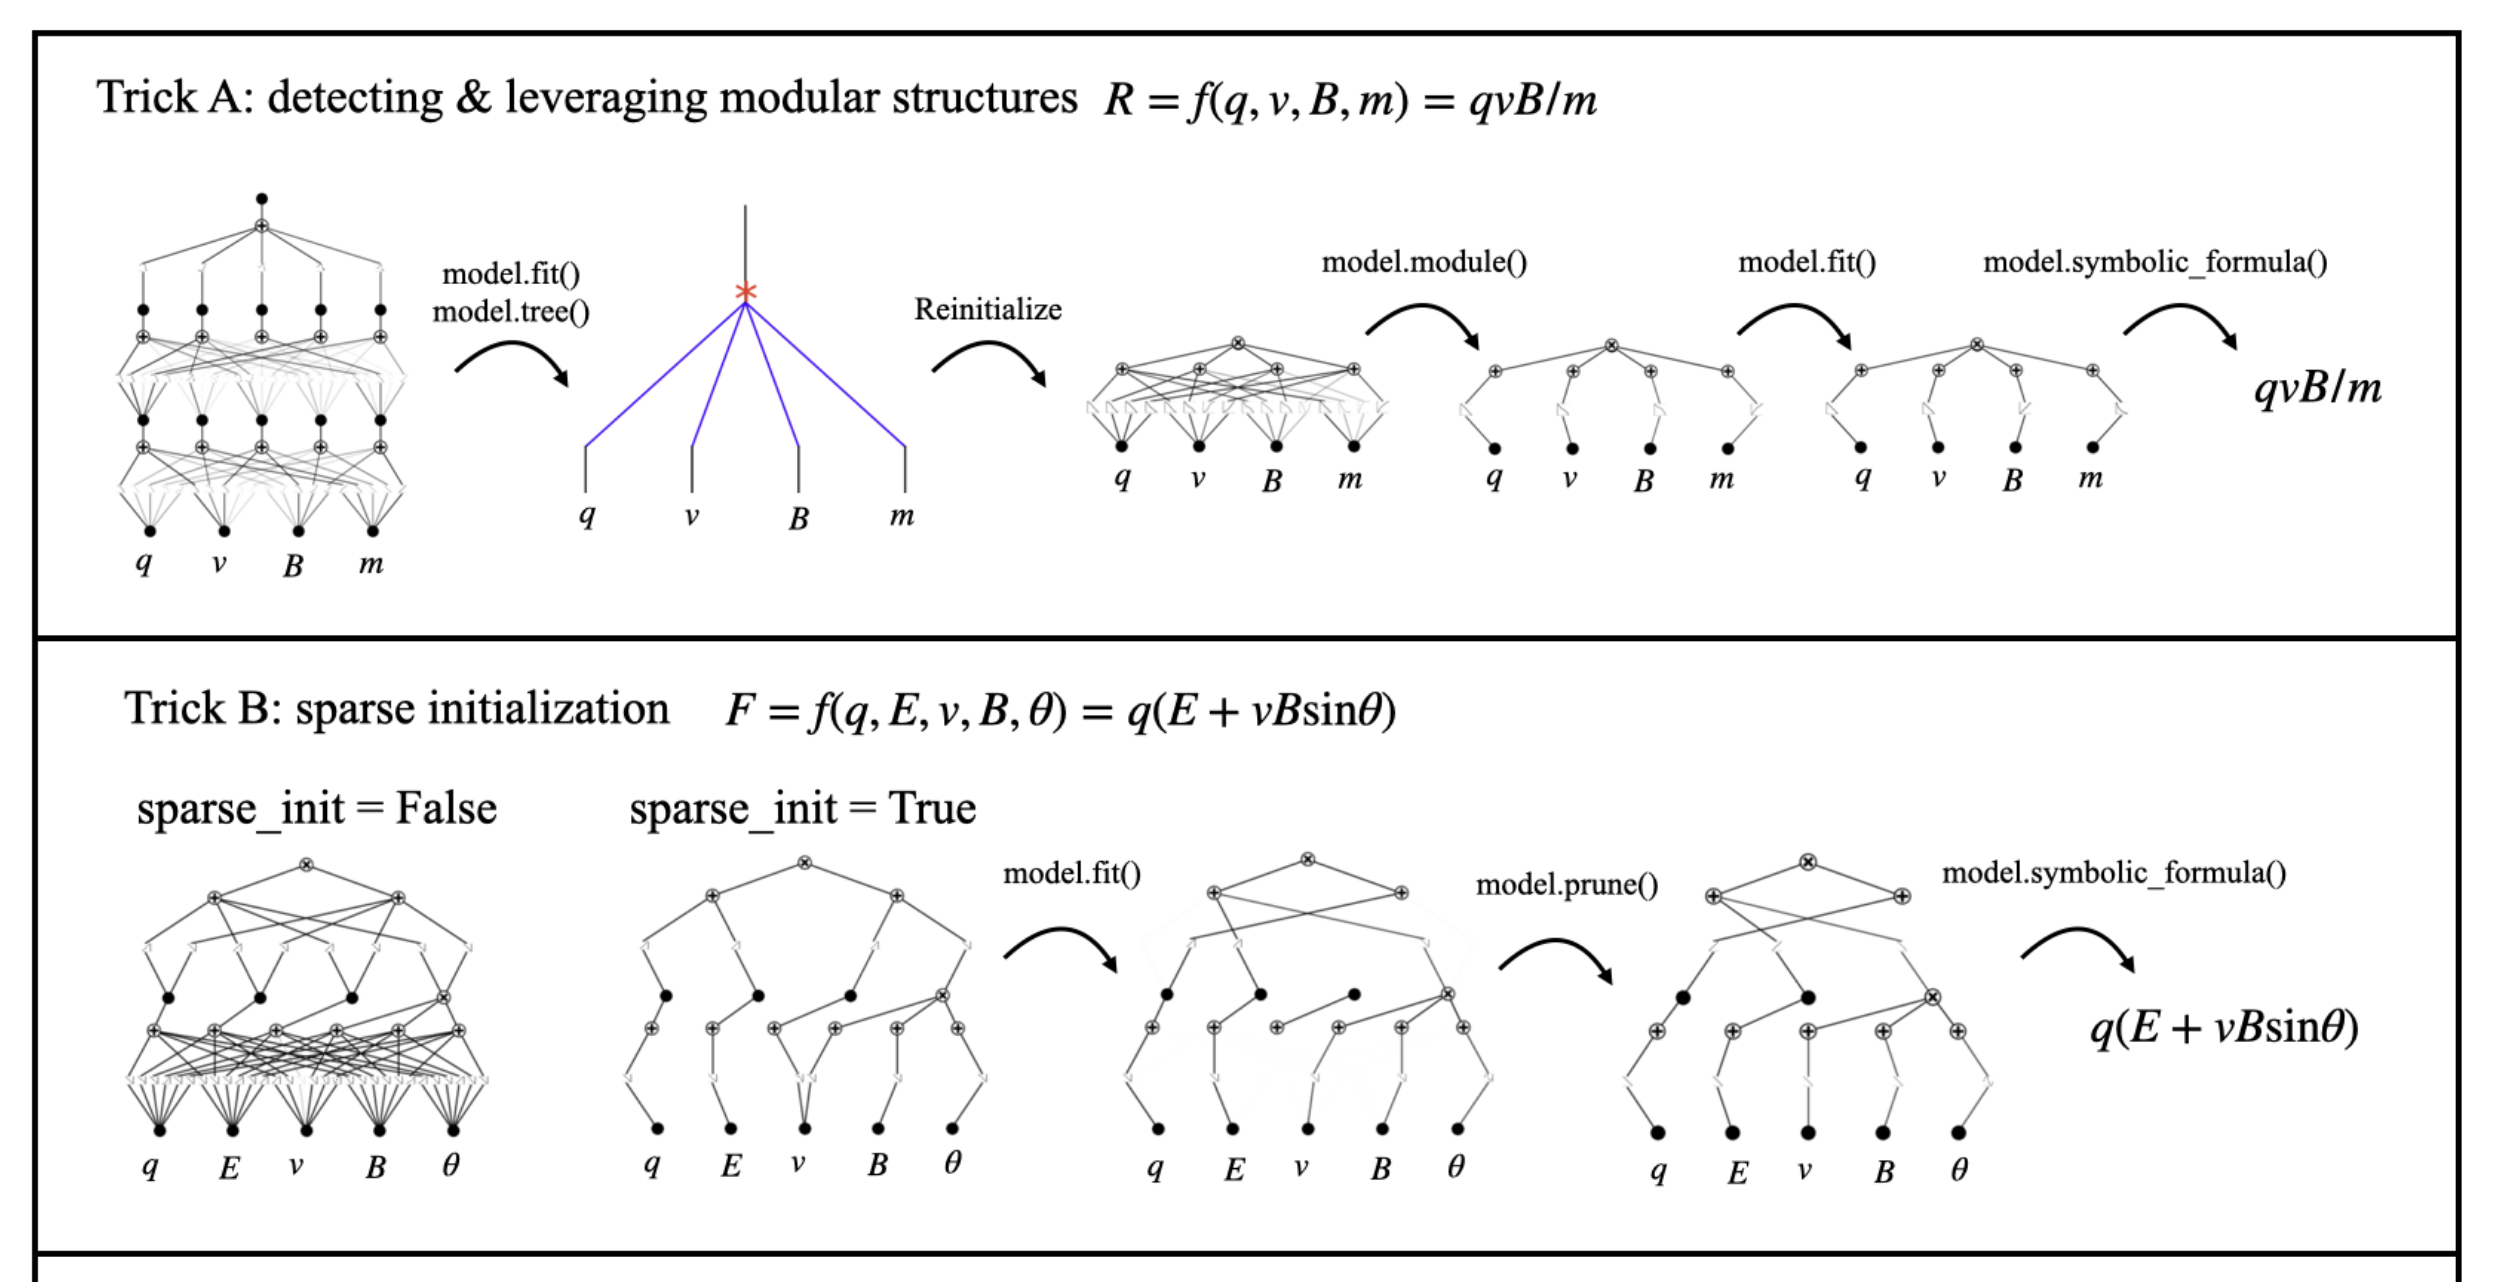
\includegraphics[width=0.95\textwidth]{images/meet_science.png}
            \caption{Приклад інтерпретації KAN мережі з роботи \cite{kan-2}.}
        \end{figure}
    \end{frame}

    \section{Конволюційні Мережі Колмогорова-Арнольда (KAN-CNN)}
    \subsection{Традиційні CNN}

    \begin{frame}{Мотивація використання CNN}
        Спробуємо ``розгорнути'' зображення $630 \times 360$ у вектор та під'єднаємо 
        до MLP. Оцінимо кількість вхідних параметрів:

	    \begin{figure}
        \centering
            
\includegraphics[width=0.73\textwidth]{images/cnn_motivation.png}
        \end{figure}
	\end{frame}

    \begin{frame}[fragile]{Конволюційна Нейронна Мережа (CNN)}
        \begin{definition}
            Нехай $\boldsymbol{X} \in \mathbb{R}^{W \times H \times C}$ ---
            набір з $C$ зображень $W \times H$, та $\boldsymbol{K} \in
            \mathbb{R}^{f \times f \times C \times C'}$ --- набір з $C'$
            фільтрів $f \times f \times C$. Тоді, згорткою з нелінійністю $\phi$
            та страйдом $s$ визначимо $\boldsymbol{Y} \in \mathbb{R}^{\frac{W}{s} \times
            \frac{H}{s} \times C'}$:
            \begin{equation*}
                \textcolor{blue}{Y_{i,j,k} = \phi\left(\sum_{u=0}^{f-1} \sum_{v=0}^{f-1} \sum_{c=0}^{C-1} X_{i+u,j+v,c} K_{u,v,c,k} + \beta_{i,j,k}\right).}
            \end{equation*}
        \end{definition}
        \vspace{-10px}
        \small
        \begin{figure}
            \[
            \left[\begin{array}{ccccccc}
            0 & 1 & 1 & \mymark{TL1}{1}\mysmall{1} & 0\mysmall{0} & \mymark{TR1}{0}\mysmall{1} & 0\\
            0 & 0 & 1 &               1\mysmall{0} & 1\mysmall{1} &               0\mysmall{0} & 0\\
            0 & 0 & 0 & \mymark{BL1}{1}\mysmall{1} & 1\mysmall{0} & \mymark{BR1}{1}\mysmall{1} & 0\\
            0 & 0 & 0 & 1 & 1 & 0 & 0\\
            0 & 0 & 1 & 1 & 0 & 0 & 0\\
            0 & 1 & 1 & 0 & 0 & 0 & 0\\
            1 & 1 & 0 & 0 & 0 & 0 & 0\\
            \end{array}\right]
            \star
            \left[\begin{array}{ccc}
            \mymark{TL2}{1} & 0 & \mymark{TR2}{1}\\
            0  & 1 &              0 \\
            \mymark{BL2}{1} & 0 & \mymark{BR2}{1}
            \end{array}\right]
            =
            \left[\begin{array}{ccccccc}
            1 & 4 & 3 & \mymark{C}{4} & 1\\
            1 & 2 & 4 & 3 & 3\\
            1 & 2 & 3 & 4 & 1\\
            1 & 3 & 3 & 1 & 1\\
            3 & 3 & 1 & 1 & 0
            \end{array}\right]
            \]
            \begin{tikzpicture}[overlay, remember picture,
                myedge1/.style={dashed, opacity=.3, blue},
                myedge2/.style={dashed, opacity=.3, green!40!black}]

            %% Draw boxes
            \draw[red, fill=red, fill opacity=.1, very thick]   (TL1.north west) rectangle (BR1.south east);
            \draw[blue, fill=blue, fill opacity=.1, very thick] (TL2.north west) rectangle (BR2.south east);
            \draw[green!60!black, fill=green, fill opacity=.1, very thick] (C.north west) rectangle (C.south east);

            %% Draw blue lines
            \draw[myedge1] (TL1.north west) -- (TL2.north west);
            \draw[myedge1] (BL1.south west) -- (BL2.south west);
            \draw[myedge1] (TR1.north east) -- (TR2.north east);
            \draw[myedge1] (BR1.south east) -- (BR2.south east);

            %% Draw green lines
            \draw[myedge2] (TL2.north west) -- (C.north west);
            \draw[myedge2] (BL2.south west) -- (C.south west);
            \draw[myedge2] (TR2.north east) -- (C.north east);
            \draw[myedge2] (BR2.south east) -- (C.south east);
            \end{tikzpicture}
            \label{fig:conv_example}
        \end{figure}
    \end{frame}

    \begin{frame}[fragile]{Приклад: Фільтри Собеля}
        \begin{tikzpicture}
            \node[anchor=center,inner sep=0](raw1) at (0,0) {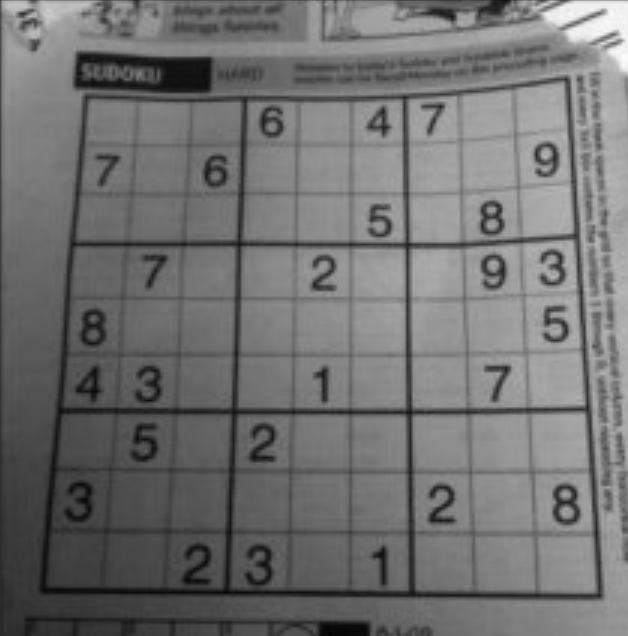
\includegraphics[width=0.3\textwidth]{images/raw.png}};
            \node[anchor=center,inner sep=0] at (2.15,-3.3) {$*$};
            \node[anchor=center,inner sep=0] at (5.8,-3.3) {$=$};
            \node[anchor=center,inner sep=0](sobel_x) at (4,0) {$\underbrace{\begin{bmatrix}
                +1 & 0 & -1 \\
                +2 & 0 & -2 \\
                +1 & 0 & -1
            \end{bmatrix}}_{\text{$x$ Sobel kernel}}$};
            \node[anchor=center,inner sep=0](img_x) at (8,0) {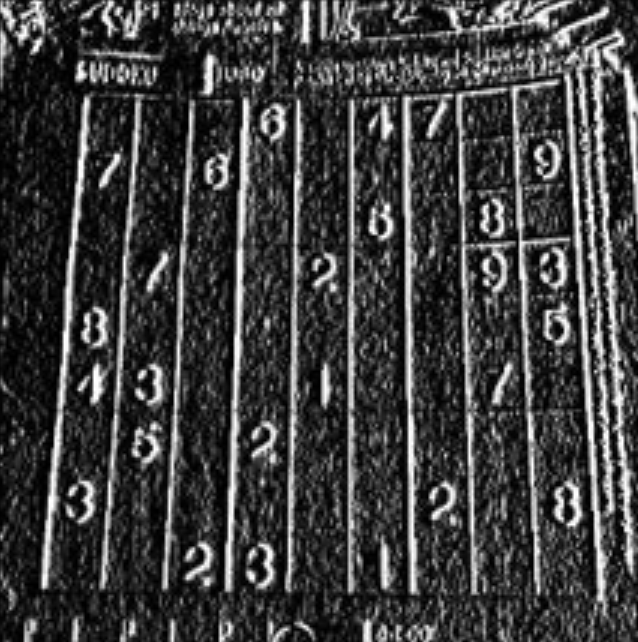
\includegraphics[width=0.3\textwidth]{images/sobel_x.png}};


            \node[anchor=center,inner sep=0](raw1) at (0,-3.5) {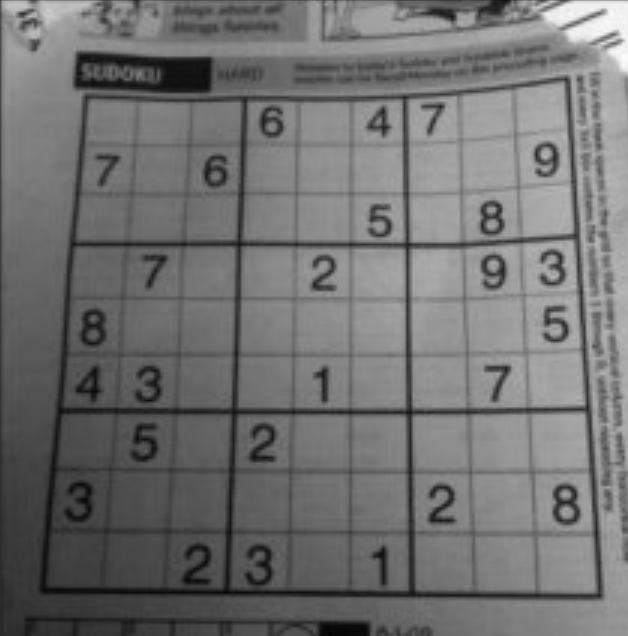
\includegraphics[width=0.3\textwidth]{images/raw.png}};
            \node[anchor=center,inner sep=0] at (2.15,0.2) {$*$};
            \node[anchor=center,inner sep=0] at (5.8,0.2) {$=$};
            \node[anchor=center,inner sep=0](sobel_x) at (4,-3.5) {$\underbrace{\begin{bmatrix}
                +1 & +2 & +1 \\
                0 & 0 & 0 \\
                -1 & -2 & -1
            \end{bmatrix}}_{\text{$y$ Sobel kernel}}$};
            \node[anchor=center,inner sep=0](img_x) at (8,-3.5) {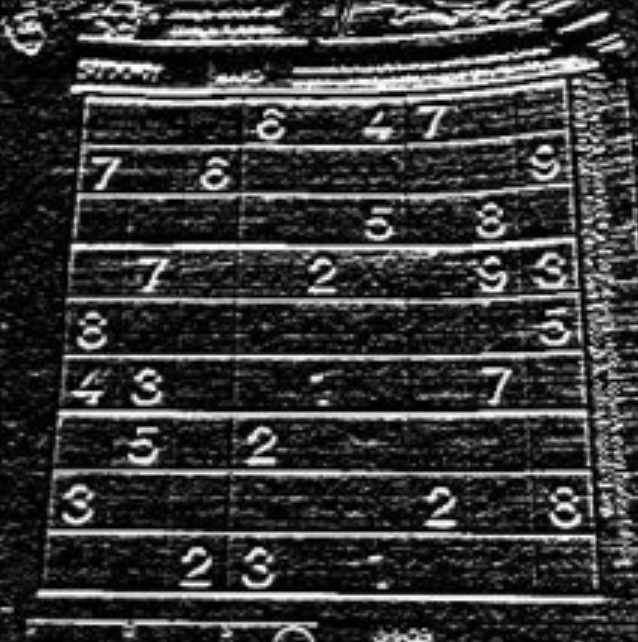
\includegraphics[width=0.3\textwidth]{images/sobel_y.png}};
        \end{tikzpicture}
    \end{frame}

    \subsection{Згортки Колмогорова-Арнольда}
    \begin{frame}[fragile]{Згортка Колмогорова-Арнольда}
        \begin{definition}
            Нехай $\boldsymbol{X} \in \mathbb{R}^{W \times H \times C}$ --- набір з $C$
            зображень (кількість каналів) розміру $W \times H$, та $\boldsymbol{K} \in
            \mathcal{F}^{f \times f \times C \times C'}$ --- набір з $C'$ фільтрів
            (ядер) розміру $f \times f \times C$, що складаються з параметризованих
            сплайнів. Тоді, результатом згортки буде нове зображення $\boldsymbol{Y} \in
            \mathbb{R}^{W \times H \times C}$:
            \begin{equation*}
                \textcolor{purple}{Y_{i,j,k} = \sum_{u=0}^{f-1} \sum_{v=0}^{f-1} \sum_{c=0}^{C'-1} \phi_{u,v,c,k}(X_{i+u,j+v,k})},
            \end{equation*}
            де $\phi_{\boldsymbol{i}}(x) =
            \omega_{\boldsymbol{i},\beta}\beta(x)+\beta_{\boldsymbol{i},S}
            \sum_j c_{\boldsymbol{i},j}B_j(x)$, $\beta(x)=x\sigma(x)$.
        \end{definition}
        \vspace{-10px}
        \scriptsize\begin{figure}
        \noindent
            \begin{minipage}{0.48\linewidth}
            \textcolor{blue}{
            \begin{equation*}
            \boldsymbol{K}_{\text{MLP}} = \begin{bmatrix}
                k_{1,1} & \cdots & k_{1,f} \\
                \vdots & \ddots & \vdots \\
                k_{f,1} & \cdots & k_{f,f}
            \end{bmatrix} \in \mathbb{R}^{f \times f}
            \end{equation*}
            MLP згортка $f \times f$, складається з $f^2$ параметрів $k_{i,j} \in \mathbb{R}$.}
            \end{minipage}
            \hfill
            \begin{minipage}{0.48\linewidth}
            \textcolor{purple}{
            \begin{equation*}
            \boldsymbol{K}_{\text{KAN}} = \begin{bmatrix}
                \phi_{1,1}(x) & \cdots & \phi_{1,f}(x) \\
                \vdots & \ddots & \vdots \\
                \phi_{f,1}(x) & \cdots & \phi_{f,f}(x)
            \end{bmatrix} \in \mathcal{F}^{f \times f}
            \end{equation*}
            KAN згортка $f \times f$, складається з $f^2$ функцій
            $\phi_{\boldsymbol{i}}(x)=\omega_{\boldsymbol{i},\beta}\beta(x)+\omega_{\boldsymbol{i},S} S(x)$.}
            \end{minipage}
            \caption{Порівняння між звичайною згорткою та згорткою Колмогорова-Арнольда.}
            \label{fig:kan_conv}
        \end{figure}
    \end{frame}

    \begin{frame}{Переваги KAN CNN}
        \textcolor{blue}{Традиційні CNN} можуть виділяти лише лінійні 
        ознаки зображення, що вимагає великої кількості шарів для 
        побудови складних ознак. 
        
        \textcolor{purple}{KAN CNN} можуть виділяти більш складні 
        залежності по лише одному шару. Наприклад, наступна функція 
        може бути апроксимована лише одним шаром KAN CNN:
        \begin{equation*}
            \phi_{i,j}(x) = \begin{cases}
                \alpha_{\text{bright}}\cdot x, & \text{якщо } x \geq \tau_{i,j}, \\
                \alpha_{\text{dark}}\cdot x, & \text{інакше.}
            \end{cases}
        \end{equation*}
    \end{frame}

    \section{Експеримент}

    \begin{frame}{MNIST Датасет}
        \begin{figure}
		\centering
		\begin{tikzpicture}
			% Define grid and spacing size
			\def\gridsize{3}
			\def\xspacing{3} % Horizontal spacing
			\def\yspacing{2} % Vertical spacing
			
			% Loop to create 3x3 grid with predictions
			\foreach \row in {1,2,3} {
				\foreach \col in {1,2,3} {
			
					% Calculate image index for sample prediction (0-9, can be random or set)
					\pgfmathtruncatemacro{\digitindex}{(\row-1)*\gridsize + \col - 1}

					% Placeholder integer predictions (customize as needed)
					\pgfmathtruncatemacro{\prediction}{mod(\digitindex, 10)} % Dummy prediction for illustration
					
					% Position of each MNIST image
					\node[draw, minimum size=1cm, inner sep=0pt] (img\row\col) at (\col*\xspacing, -\row*\yspacing)
					{\includegraphics[width=1.75cm]{../figures/mnist/digit\digitindex.png}};
			
					% Prediction label with actual prediction value next to each digit
					\node[right=0.5cm of img\row\col] (pred\row\col) {\textbf{\prediction}};
			
					% Arrow pointing from image to prediction
					\draw[->, thick] (img\row\col) -- node[above] {\( f \)} (pred\row\col);
				}
			}
		\end{tikzpicture}
		\caption{Приклад класифікації цифр. Маючи зображення $X \in \mathbb{R}^{W \times H}$, наша функція дає дискретне передбачення $f(X) \in \{0,\dots,9\}$ --- цифра, яка зображена на зображенні $X$.}
		\label{fig:digits}
	\end{figure}
    \end{frame}

    \begin{frame}
 \begin{figure}
    \centering
    \tikzset{
        base/.style={
            draw,
            rectangle,
            minimum width=5cm,
            minimum height=1cm,
            very thick,
            rounded corners=7.5pt
        },
        maxpool/.style={
            base,
            fill=orange!10,
            draw=orange!90!black
        },
        kanconv/.style={
            base,
            fill=blue!10,
            draw=blue!80!black
        },
        fc/.style={
            base,
            fill=green!10,
            draw=green!70!black
        }
    }
    \begin{tikzpicture}[scale=0.6, transform shape]
        % Input
        \node[base] (input) {\textbf{Вхід}};
        \node[left=1cm of input, thick] (image) {
\includegraphics[width=1.75cm]{../figures/mnist/digit5.png}};
        \draw[thick, line width=1.5pt, -{Stealth[length=7pt, width=7pt]}] (image) -- (input);
        \node[above=0.1cm of image] {\textcolor{gray}{$\boldsymbol{X} \in \mathbb{R}^{28 \times 28 \times 1}$}};

        \node[kanconv, below=0.1cm of input] (conv1) {KANConv, $3 \times 3$, $8$};
        \node[right=0.3cm of conv1] {\textcolor{gray}{720 параметрів}};
        
        \node[maxpool, below=0.1cm of conv1] (maxpool1) {MaxPool2D, $2 \times 2$};
        
        \node[kanconv, below=0.1cm of maxpool1] (conv2) {KANConv, $3 \times 3$, $16$};
        \node[right=0.3cm of conv2] {\textcolor{gray}{13.8k параметрів}};
        
        \node[maxpool, below=0.1cm of conv2] (maxpool2) {MaxPool2D, $2 \times 2$};
        
        \node[kanconv, below=0.1cm of maxpool2] (conv3) {KANConv, $3 \times 3$, $32$};
        \node[right=0.3cm of conv3] {\textcolor{gray}{41.5k параметрів}};
        
        \node[maxpool, below=0.1cm of conv3] (maxpool3) {MaxPool2D, $2 \times 2$};
        
        \node[fc, below=0.9cm of maxpool3] (fc) {$7 \cdot 7 \cdot 32$ нейронів};
        
        \node[fc, below=0.1cm of fc] (fc2) {Лінійний шар, $1568 \times 10$};
        \node[left=0.3cm of fc2] {\textcolor{gray}{15.4k параметрів}};
        \node[right=2.25cm of fc2] (output-label) {\textcolor{gray}{$\boldsymbol{y} \in \mathbb{R}^{10}$}};
        \draw[thick, line width=1.5pt, -{Stealth[length=7pt, width=7pt]}] (fc2) -- (output-label) node[midway, above] {Softmax};

        % Draw stealth arrows 
        % \draw[thick, line width=1.5pt, -{Stealth[length=7pt, width=7pt]}] (input) -- (conv1);
        % \draw[thick, line width=1.5pt, -{Stealth[length=7pt, width=7pt]}] (conv1) -- (maxpool1);
        % \draw[thick, line width=1.5pt, -{Stealth[length=7pt, width=7pt]}] (maxpool1) -- (conv2);
        % \draw[thick, line width=1.5pt, -{Stealth[length=7pt, width=7pt]}] (conv2) -- (maxpool2);
        % \draw[thick, line width=1.5pt, -{Stealth[length=7pt, width=7pt]}] (maxpool2) -- (conv3);
        % \draw[thick, line width=1.5pt, -{Stealth[length=7pt, width=7pt]}] (conv3) -- (maxpool3);
        % \draw[thick, line width=1.5pt, -{Stealth[length=7pt, width=7pt]}] (maxpool3) -- (conv4);
        \draw[thick, line width=1.5pt, -{Stealth[length=7pt, width=7pt]}] (maxpool3) -- (fc) node[midway, right] {Flatten};
        \end{tikzpicture}
        \caption{Архітектура нейронної мережі на основі конволюційних шарів 
        Колмогорова-Арнольда (CKAN).}
        \label{fig:kan-arch}
    \end{figure}       
    \end{frame}

    \begin{frame}{Тренування}
        \begin{center}
            \url{https://github.com/ZamDimon/convolutional-kan}
        \end{center}
        \begin{figure}
            \centering
            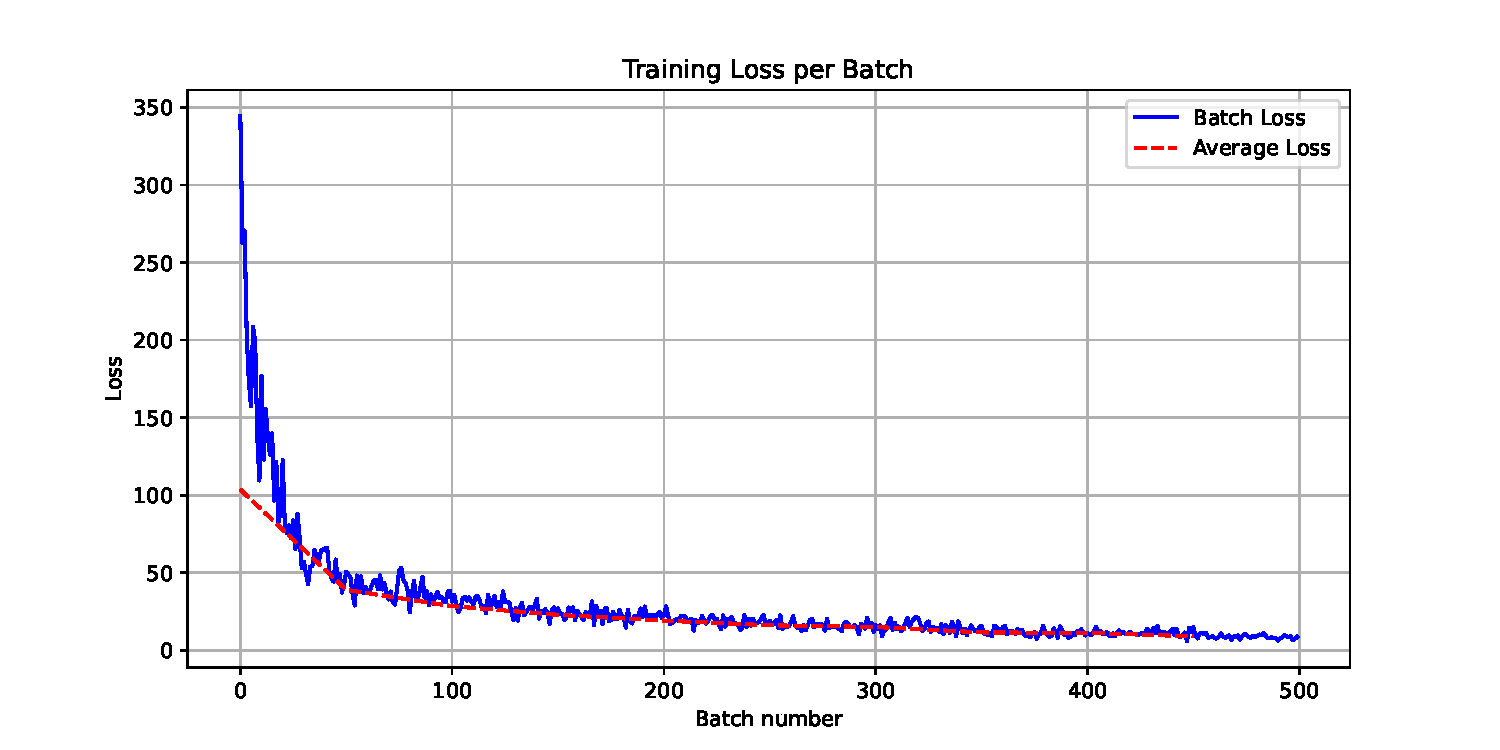
\includegraphics[width=\textwidth]{../figures/batch_loss_curve.pdf}
            \caption{Крива тренування нейронної мережі на основі конволюційних шарів 
            Колмогорова-Арнольда (CKAN).}
            \label{fig:train-curve}
        \end{figure}
    \end{frame}

    \begin{frame}{Висновки}
        \begin{itemize}
            \item Досягнута точність на тестовому наборі MNIST \textbf{87.8\%}. 
            \item $F_1$ міра дорівнює \textbf{87.2\%}.
            \item Час тренування приблизно $\times 50$ в порівнянні з 
            традиційними CNN: процес тренування дуже довгий, як і зазначено в 
            оригінальній роботі \cite{kan}. Причина --- погана паралелізованість 
            $B$-сплайнів.
            \item Проте, за такої саме MLP архітектури з класичними
            \texttt{Conv2D} шарами, точність MLP моделі була близько $85\%$ --- отже,
            KAN конволюції несуть більше інформації.
        \end{itemize}

        \begin{alertblock}{Висновок}
            Конволюційні шари Колмогорова-Арнольда (KAN-CNN) можуть бути
            використані для побудови глибоких нейронних мереж, але поки вони
            дуже повільні та нестабільні. Потрібно більше досліджень для
            оптимізації їх тренування.
        \end{alertblock}
    \end{frame}

    \begin{frame}[allowframebreaks]{Література}
        % This prints the bibliography on the slide
        \printbibliography
    \end{frame}

    \begin{frame}[plain, standout]
      \centering
      \LARGE
      \textbf{Дякую за Вашу Увагу!} \\
      
      \vspace{0.2cm} \Huge \ding{170} \large \\
    \end{frame}

    \subsection*{Математичний додаток}

    \begin{frame}{Щільність у функціональному просторі}
        \begin{definition}
            Нехай $(\mathcal{F}, \|\cdot\|)$ --- нормований простір. Підмножина
            $\mathcal{G} \subset \mathcal{F}$ називається \textbf{щільною} в
            $\mathcal{F}$, якщо замикання $\mathcal{G}$ збігається з
            $\mathcal{F}$, тобто $\overline{\mathcal{G}} = \mathcal{F}$.
        \end{definition}

        \begin{block}{Еквівалентне визначення}
             Для будь-якої функції $f \in \mathcal{F}$ та для будь-якого
             $\varepsilon > 0$, існує функція $g \in \mathcal{G}$ така, що $\|f
             - g\| < \varepsilon$.
        \end{block}
    \end{frame}

    \begin{frame}{Теорема Вейєрштрасса про апроксимацію}
        \begin{theorem}[Weierstrass, 1885]
            Нехай $f \in \mathcal{C}([a,b])$ --- неперервна функція на замкненому інтервалі. Для будь-якого $\varepsilon > 0$ існує поліном $P(x)$ такий, що для всіх $x \in [a,b]$ виконується нерівність:
            $$ |f(x) - P(x)| < \varepsilon $$
        \end{theorem}
        
        \begin{block}{Висновок}
            Множина всіх поліноміальних функцій $\mathbb{R}[x]$ є щільною у просторі неперервних функцій $\mathcal{C}([a,b])$ відносно норми рівномірної збіжності $\|\cdot\|_{\infty}$.
            $$ \|\phi\|_{\infty} = \sup_{x \in [a,b]} |\phi(x)| $$
        \end{block}
    \end{frame}

    \begin{frame}{Визначення: Простір Лебега $L^p$}
        \begin{definition}
            Нехай $(\mathcal{X}, \mathcal{F}, \mu)$ --- простір з мірою. Для $p
            \in [1, \infty)$, \textbf{простір Лебега} $L^p(\mathcal{X})$ --- це
            множина всіх $\mathcal{F}$-вимірних функцій $f: \mathcal{X} \to
            \mathbb{R}$, для яких скінченна $L^p$-норма:
            $$ \|f\|_{p} := \left( \int_{\mathcal{X}} |f|^p \,d\mu \right)^{1/p}
            < \infty $$ Для $p=\infty$, $L^\infty(\mathcal{X})$ --- це простір
            обмежених функцій з нормою:
            $$ \|f\|_{\infty} := \underset{x \in \mathcal{X}}{\sup} |f(x)| < \infty$$
        \end{definition}
    \end{frame}
\end{document}